\documentclass[12pt]{beamer}
%\includeonlyframes{current}

\mode<presentation>{\usetheme{Warsaw}}
\setbeamertemplate{footline}[frame number]
\AtBeginSection[]{
\begin{frame}<beamer>{Outline}
	\tableofcontents[currentsection]
\end{frame}
}

\usepackage[english]{babel}
\usepackage{times}
\usepackage{url}
\usepackage{graphicx}
\usepackage{hhline}
\usepackage{array}
\usepackage{colortbl}
\usepackage{changepage}

\newcommand{\key}[1]{{\color{blue}#1}}
\newcommand{\cmnt}[1]{{\color{gray}#1}}
\newcommand{\str}[1]{{\color{green!50!black}#1}}
\newcommand{\num}[1]{{\color{green!55!blue}#1}}
\newcommand{\defn}[1]{{\color{purple}#1}}
\newcommand{\SC}[1]{\mbox{\sc#1}}
\newcommand{\EM}[1]{\mbox{\em#1}}
\newcommand{\tab}{\hspace{1em}}

\newcommand{\AEM}[1]{\alert{\EM{#1}}}

\title{Probabilistic Reasoning}
\subtitle{Introduction to Artificial Intelligence}
\author{Steven Bethard}
\institute{
  Department of Computer Science\\
  University of Colorado
}
\date{CSCI 3202}


\begin{document}

\begin{frame}
	\titlepage
\end{frame}

\section{Bayesian Networks}
\subsection{Bayesian Network Basics}
\begin{frame}{Bayesian Networks}
	\begin{block}{Definition}
		A \alert{Bayesian Network} is a data structure for representing independence relations among random variables
	\end{block}
	\pause
	\medskip
	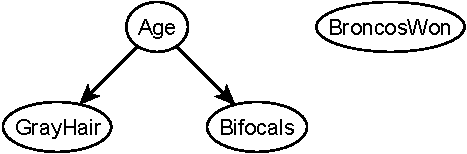
\includegraphics[height=1in]{age_broncos_net} \\
	\medskip
	\pause
	$
	\begin{array}{ll}
	\lefteqn{P(\EM{Age}, \EM{GrayHair}, \EM{Bifocals}, \EM{BroncosWon}) = \mbox{}}\\ 
	& P(\EM{Age}, \EM{GrayHair}, \EM{Bifocals})P(\EM{BroncosWon})
	\end{array}
	$
	\pause
	\smallskip
	$
	\begin{array}{ll}
	\lefteqn{P(\EM{GrayHair},\EM{Bifocals}|\EM{Age}) = \mbox{}}\\ 
	& P(\EM{GrayHair}|\EM{Age})P(\EM{Bifocals}|\EM{Age})
	\end{array}
	$ \\
\end{frame}
\begin{frame}{Bayesian Networks}
	\begin{block}{Components}
		\begin{itemize}
			\item Random variables (nodes)
			\item Directed links from \EM{parent} nodes to \EM{child} nodes
			\item $\mathbf{P}(X_{i}|\EM{Parents}(X_{i}))$ tables for each node
			\item Links form no cycles
		\end{itemize}
	\end{block}
	\pause
	\begin{block}{Intuitions}
		\begin{itemize}
			\item Links indicate \emph{direct} influence
			\item Causes usually near top
			\item Effects usually near bottom
		\end{itemize}
	\end{block}
\end{frame}
\begin{frame}{Full Bayesian Network Example}
	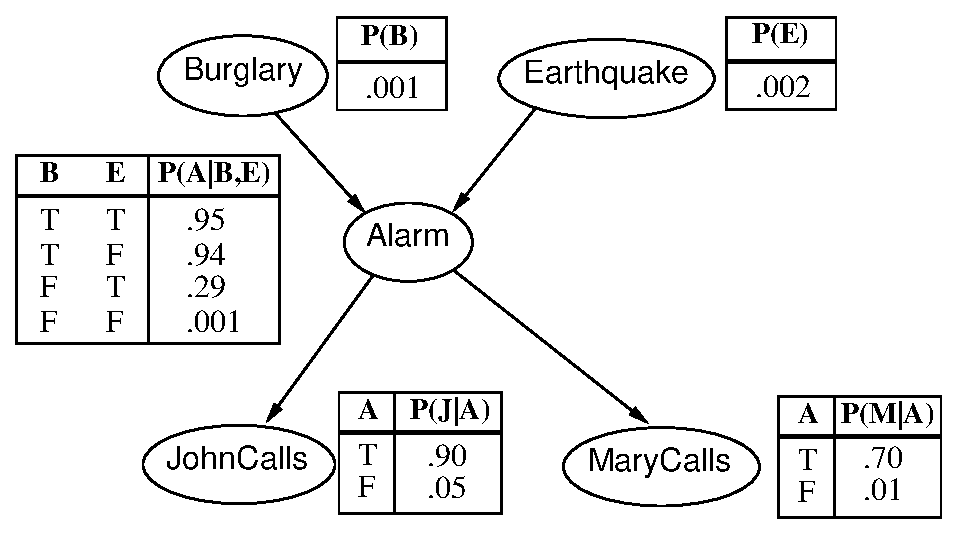
\includegraphics[width=4.2in]{burglary_network}
\end{frame}


\subsection{The Full Joint Distribution}
\begin{frame}{Representing the Full Joint Distribution}
	\begin{block}{Key Formula}
		$P(x_{1},\ldots,x_{n}) = \prod\limits_{i=1}^{n}{P(x_{i}|\EM{parents}(X_{i}))}$
	\end{block}
	\begin{block}{Example}
		$
		\begin{array}{lll}
			\lefteqn{P(j, m, a, \lnot b, \lnot e)}
			\\
			& = & \pause
			      P(j|\EM{parents}(j)) \cdot
			      P(m|\EM{parents}(m)) \cdot
			      \ldots
			\\
			& = & \pause
			      P(j|a) \cdot
			      P(m|a) \cdot
			      P(a|\lnot b, \lnot e) \cdot
			      P(\lnot b) \cdot
			      P(\lnot e)
			\\
			& = & \pause
			      0.90 \cdot
			      0.70 \cdot
			      0.001 \cdot
			      0.999 \cdot
			      0.998
			\\
			& = & \pause
			      0.00062
		\end{array}
		$
	\end{block}
\end{frame}
\begin{frame}{A Simple Inference Algorithm}
	\begin{block}{Goal: Answer Queries}
		\begin{itemize}
			\item One query variable given some evidence
			\item $\mathbf{P}(X|y_{1},\ldots,y_{n})$
		\end{itemize}
	\end{block}
	\pause
	\begin{block}{Solution: Enumeration}
		$
		\begin{array}{@{}lll@{}}
			\lefteqn{\mathbf{P}(X|y_{1},\ldots,y_{n})} \\
			& = & \alpha\mathbf{P}(X,y_{1},\ldots,y_{n}) \\
			& = & \alpha\sum\limits_{z_{1},\ldots,z_{k} \in \mathbf{\overline{XY}}}
			      {\mathbf{P}(X,y_{1},\ldots,y_{n},z_{1},\ldots,z_{k})} \\
			& = & \alpha\sum\limits_{z_{1},\ldots,z_{k} \in \mathbf{\overline{XY}}}
			      {\mathbf{P}(X|\ldots)
			       P(y_{1}|\ldots)
			       \ldots
			       P(z_{k}|\ldots)} \\
		\end{array}
		$
	\end{block}
\end{frame}
\begin{frame}{Worst Case for Simple Inference Algorithm}
	\begin{block}{Enumeration Formula}
		$
		\mathbf{P}(X|y_{1},\ldots,y_{n}) = 
		\alpha\sum\limits_{z_{1},\ldots,z_{k} \in \mathbf{\overline{XY}}}
		          {\mathbf{P}(X|\mbox{\scriptsize\ldots})
		           P(y_{1}|\mbox{\scriptsize\ldots})
		           \ldots
		           P(z_{k}|\mbox{\scriptsize\ldots})}
		$
	\end{block}
	\pause
	\begin{columns}
		\begin{column}{1.5in}
			\begin{center}
				\includegraphics[height=1.5in]{fully_connected_net}
				\\
				\smallskip
				Query: $P(X_{5})$
			\end{center}
		\end{column}
		\pause
		\begin{column}{2.5in}
			\begin{block}{Worst Case in General}
				\begin{itemize}
					\item $\approx n$ parents per node
					\item $\approx n$ variables not in query
					\item $d$ values per variable
				\end{itemize}
				Time Complexity: \pause $O(nd^{n})$
			\end{block}
		\end{column}
	\end{columns}
\end{frame}


\subsection{Constructing Bayesian Networks}
\begin{frame}{Avoiding Fully Connected Networks}
	\begin{block}{Principles}
		\begin{enumerate}
			\item Add root causes
			\item\label{add-leaf-effects} Add variables directly influenced by leaves
			\item If variables left, goto \ref{add-leaf-effects}
		\end{enumerate}
	\end{block}
	\medskip
	\begin{columns}
		\begin{column}{2.2in}
			\uncover<2->{
			Good:
			\\
			\footnotesize \EM{Age}, \EM{GrayHair}, \EM{Bifocals}, \EM{ReadDist}} \\
			\centering
			\only<-3>{\invisible<-2>{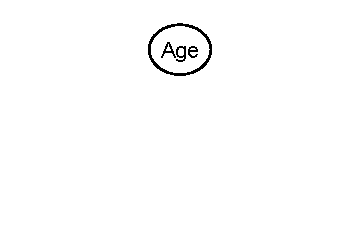
\includegraphics[height=1.2in]{age_hair_vision_1}}}%
			\only<4>{\includegraphics[height=1.2in]{age_hair_vision_2}}%
			\only<5>{\includegraphics[height=1.2in]{age_hair_vision_3}}%
			\only<6->{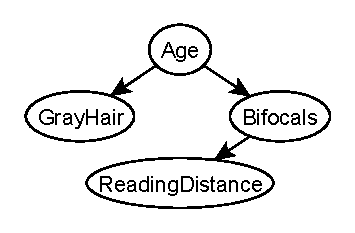
\includegraphics[height=1.2in]{age_hair_vision_4}}%
		\end{column}
		\begin{column}{2.2in}
			\uncover<7->{
			Bad:
			\\
			\footnotesize \EM{ReadDist}, \EM{GrayHair}, \EM{Bifocals}, \EM{Age}} \\
			\centering
			\only<-8>{\invisible<-7>{\includegraphics[height=1.2in]{vision_hair_age_1}}}%
			\only<9>{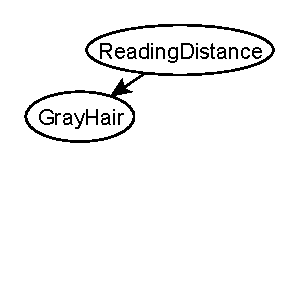
\includegraphics[height=1.2in]{vision_hair_age_2}}%
			\only<10>{\includegraphics[height=1.2in]{vision_hair_age_3}}%
			\only<11->{\includegraphics[height=1.2in]{vision_hair_age_4}}%
		\end{column}
	\end{columns}
\end{frame}
\begin{frame}{Bayesian Network Exercise}
	\begin{block}{Construct a Network}
		\begin{itemize}
			\item The fire alarm usually goes off when there's a fire
			\item When the alarm rings everyone usually exits together
			\item Most of the time there's smoke when there's a fire
			\item Someone sometimes pulls the fire alarm ``as a joke''
			\item The fire trucks usually come when the alarm goes off
			\item Sometimes everyone exits together for a picnic
		\end{itemize}
	\end{block}
\end{frame}
\begin{frame}{Bayesian Network Exercise}
	One possible solution:
	\begin{center}
		\includegraphics[height=2in]{fire_alarm}
	\end{center}
\end{frame}


\section{Efficient Exact Inference}
\subsection{Moving Summation Terms}
\begin{frame}{Drawbacks of Simple Enumeration}
	\begin{block}{Recall: Simple Enumeration}
		Time Complexity: $O(nd^{n})$
	\end{block}
	\pause
	\begin{block}{Example}
		$
		\begin{array}{@{}lll@{}}
		P(b|j,m) & = & \alpha\sum\limits_{e}\sum\limits_{a}P(b)P(e)P(a|b,e)P(j|a)P(m|a) \\
		         & = & \alpha(P(b)P(e)P(a|b,e)P(j|a)P(m|a) + \mbox{}\\
		         &   &   \tab P(b)P(e)P(\lnot a|b,e)P(j|\lnot a)P(m|\lnot a) + \mbox{}\\
		         &   &   \tab P(b)P(\lnot e)P(a|b,\lnot e)P(j|a)P(m|a) + \mbox{}\\
		         &   &   \tab P(b)P(\lnot e)P(\lnot a|b,\lnot e)P(j|\lnot a)P(m|\lnot a))
		\end{array}
		$
		\\
		\medskip
		\pause Problem: \pause We calculate $P(b)$, $P(e)$ and $P(\lnot e)$ many times!
	\end{block}
\end{frame}
\begin{frame}{More Intelligent Summation}
	\begin{block}{Moving Terms in Algebra}
		$
		\begin{array}{lll}
		\lefteqn{abd + abe + acf + acg} \\
		   & = & \pause a(bd + be + cf + cg) \\
		   & = & \pause a(b(d + e) + c(f + g)) \\
		\end{array}
		$
	\end{block}
	\pause
	\begin{block}{Moving Terms in Bayesian Network Calculations}
		$
		\begin{array}{lll}
		P(b|j,m) & = & \alpha\sum\limits_{e}\sum\limits_{a}P(b)P(e)P(a|b,e)P(j|a)P(m|a) \\
		         & = & \pause
		               \alpha P(b)\sum\limits_{e}\sum\limits_{a}P(e)P(a|b,e)P(j|a)P(m|a) \\
		         & = & \pause
		               \alpha P(b)\sum\limits_{e}P(e)\sum\limits_{a}P(a|b,e)P(j|a)P(m|a)
		\end{array}
		$
	\end{block}
\end{frame}

\subsection{Dynamic Programming}
\begin{frame}{Calculations through Depth First Search}
	Example formula: \\
	\tab $P(b|j,m) = \alpha P(b)\sum\limits_{e}P(e)\sum\limits_{a}P(a|b,e)P(j|a)P(m|a)$ \\
	\pause
	\bigskip
	Example tree: \\
	\vspace{-2em}
	\begin{center}
		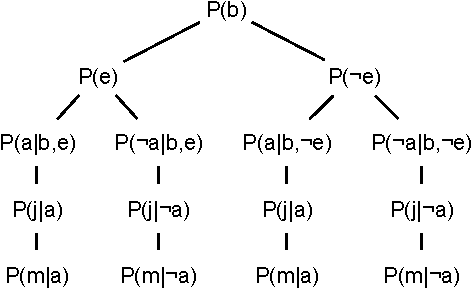
\includegraphics[height=2in]{summation_tree}
	\end{center}
\end{frame}
\begin{frame}{Eliminating More Redundancies}
	\begin{columns}
		\begin{column}{2.2in}
			\begin{block}{Problem}
				\begin{itemize}
					\item Moving terms got rid of some redundancies
					\item But notice: \\
					      $P(j|a)P(m|a)$ \\
					      $P(j|\lnot a)P(m|\lnot a)$
				\end{itemize}
			\end{block}
			\begin{block}<2->{Solution}
				\begin{itemize}
					\item<3-> Dynamic programming!
					\item<4-> Store partial calculations
					\item<4-> Look up repeated terms
				\end{itemize}
			\end{block}
		\end{column}
		\begin{column}{2.4in}
			\includegraphics[width=2.4in]{summation_tree_narrow}
		\end{column}
	\end{columns}
\end{frame}

\subsection{Exact Inference Properties}
\begin{frame}{Exact Inference Properties}
	\begin{block}{Moving Summation Terms}
		Given $n$ boolean variables:
		\\ \medskip
		\begin{tabular}{ll}
			\key{Time Complexity?}  & \pause $O(2^{n})$, explores whole tree
			\\ \pause
			\key{Space Complexity?} & \pause $O(n)$, depth first search
		\end{tabular}
	\end{block}
	\pause
	\begin{block}{With Dynamic Programming}
		\begin{tabular}{@{}ll@{}}
			\lefteqn{\mbox{\key{Singly connnected networks}}} \\
			& Time and space $O(n)$ if number of parents is bounded \\
			\pause
			\lefteqn{\mbox{\key{Multiply connected networks}}} \\
			& Time and space can be as bad as $O(k^{n})$
		\end{tabular}
	\end{block}
\end{frame}


\section{Approximate Inference}
\begin{frame}{Approximate Inference}
	\begin{block}{Motivation}
		\begin{itemize}
			\item Exact inference is exponential in number of variables
			\item Sometimes an approximate result is enough
				\begin{itemize}
					\item E.g. 29.6\% vs. 30.0\% chance of rain
				\end{itemize}
		\end{itemize}
	\end{block}
	\pause
	\begin{block}{General Approach for Approximate Inference}
		\begin{itemize}
			\item Generate a bunch of full variable assignments
			\item Make sure assignments are consistent with evidence
			\item Count times $X\!=\!x$ and divide by number of samples
		\end{itemize}
	\end{block}
\end{frame}
\begin{frame}[fragile]{Generating Full Variable Assignments}
	\begin{block}{Key Ideas for Creating a Random Assignment}
		\begin{itemize}
			\item Nodes are ordered from parents to children
			\item Single nodes calculate $P(x_{i}|\EM{parents}(X_{i}))$
		\end{itemize}
	\end{block}
	\pause
	\bigskip
	\begin{adjustwidth}{-1em}{-1em}
	\begin{semiverbatim}\scriptsize\bfseries
		\key{def} \defn{prior_sample}(bayes_net):
		    \pause\cmnt{# generate a value for each variable from roots to leaves}
		    sample = []
		    \key{for} node \key{in} bayes_net:
		        \pause\cmnt{# find the values assigned to the parents}
		        parent_samples = [sample[p.index] \key{for} p \key{in} node.parents]
		        \pause\cmnt{# find the probability for this assignment from the table}
		        prob = node.get_prob(\key{True}, *parent_samples)
		        \pause\cmnt{# add True or False according to the distribution}
		        sample.append(random.random() < prob)
		    \pause\cmnt{# return the complete sample}
		    \key{return} sample
	\end{semiverbatim}
	\end{adjustwidth}
\end{frame}


\subsection{Rejection Sampling}
\begin{frame}[fragile]{Rejection Sampling}
	\begin{block}{Key Idea}
		Throw away samples inconsistent with the evidence
	\end{block}
	\medskip
	\pause
	\begin{tabular}{ll}
		Variables: & \EM{Cloudy}, \EM{Sprinkler}, \EM{Rain}, \EM{WetGrass} \\
		Query:     & $P(\EM{Rain}|\EM{Sprinkler}\!=\!\EM{true})$
	\end{tabular}
	\\
	\medskip
	$
	\begin{array}{llll|cc}
		\EM{Cloudy} & \EM{Sprinkler} & \EM{Rain}  & \EM{WetGrass} & \EM{rain} & \lnot\EM{rain} \\
		\hline
		\pause
		\EM{false}  & \EM{false}     & \EM{false} & \EM{false}    &           &            \\
		\pause
		\EM{true}   & \EM{true}      & \EM{false} & \EM{true}     &           & \pause 1   \\
		\pause
		\EM{true}   & \EM{false}     & \EM{false} & \EM{false}    &           &            \\
		\pause
		\EM{false}  & \EM{true}      & \EM{true}  & \EM{true}     & \pause 1  &            \\
		\pause
		\EM{false}  & \EM{true}      & \EM{false} & \EM{true}     &           & \pause 1
	\end{array}
	$
	\\
	\medskip
	\pause
	\tab$P(\EM{Rain}\!=\!\EM{true}|\EM{Sprinkler}\!=\!\EM{true})=\pause\frac{1}{1 + 1 + 1}=\frac{1}{3}$
\end{frame}
\begin{frame}[fragile]{Rejection Sampling Code}
	\begin{adjustwidth}{-1em}{-1em}
	\begin{semiverbatim}\scriptsize\bfseries
		\key{def} \defn{rejection_sampling}(query_var, evidence, bayes_net, samples):
		    \pause\cmnt{# generate a bunch of samples, counting query values}
		    counts = \{\key{False}: \num{0}, \key{True}: \num{0}\}
		    \key{for} _ \key{in} range(samples):
		        sample = prior_sample(bayes_net)
		        \pause\cmnt{# if the sample is consistent with the evidence, count it}
		        \key{if} all(sample[v.index] == evidence[v] \key{for} v \key{in} evidence):
		            counts[sample[query_var.index]] += \num{1}
		    \pause\cmnt{# normalize the counts and return the probabilities}
		    \key{return} normalize(counts)
		\pause
		\key{def} \defn{normalize}(counts):
		    \pause\cmnt{# divide all counts by the total}
		    total = sum(counts.values())
		    \key{for} value \key{in} counts:
		        counts[value] /= total
		    \pause\cmnt{# return the probabilities}
		    \key{return} counts
	\end{semiverbatim}
	\end{adjustwidth}
\end{frame}
\begin{frame}{Rejection Sampling Exercise}
	\begin{columns}
		\begin{column}{2.7in}
			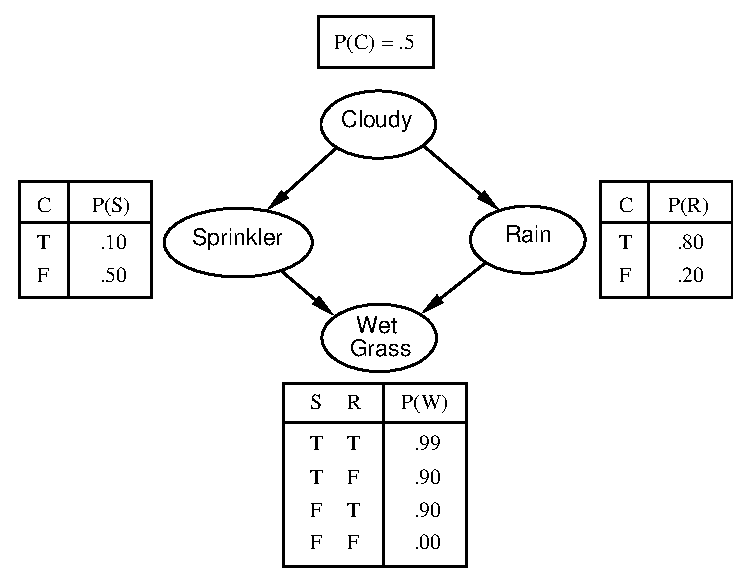
\includegraphics[width=2.7in]{rain_net}
		\end{column}
		\begin{column}{1.5in}
			\small
			Calculate: \\
			\smallskip
			\begin{tabular}{l@{}}
				$P(\EM{rain}|\EM{sprinkler})$ \\
				5 samples \\
				\EM{true} if below random
			\end{tabular} \\
			\medskip
			Random numbers: \\
			\smallskip
			$
			\begin{array}{llll}
				\parbox{.22in}{C} & \parbox{.22in}{S}            & \parbox{.22in}{R}             & WG                \\
				\hline
				\alt<2->{F}{0.6}  & \alert<8->{\alt<3->{T}{0.4}} & \alt<4->{F}{0.3}              & \alt<5->{T}{0.8} \\
				\alt<6->{F}{0.7}  & \alert<8->{\alt<6->{T}{0.3}} & \alt<6->{F}{0.8}              & \alt<6->{T}{0.6} \\
				\alt<6->{T}{0.3}  &            \alt<6->{F}{0.2}  & \alt<6->{T}{0.7}              & \alt<6->{T}{0.3}  \\
				\alt<6->{F}{0.9}  & \alert<8->{\alt<6->{T}{0.2}} & \alt<6->{F}{0.4}              & \alt<6->{T}{0.1} \\
				\alt<6->{F}{0.8}  & \alert<8->{\alt<6->{T}{0.4}} & \alert<9->{\alt<6->{T}{0.1}}  & \alt<6->{T}{0.9} \\
			\end{array}
			$ \\
			\medskip
			\uncover<7->{$P(\EM{rain}|\EM{sprinkler}) = \uncover<10->{\frac{1}{4}}$}
		\end{column}
	\end{columns}
\end{frame}
\begin{frame}{Rejection Sampling}
	\begin{block}{Properties}
		Given $n$ variables, at most $d$ parents each, $s$ samples drawn and $u$ samples used:
		\begin{itemize}
			\item Time Complexity: \pause $O(nds)$
			\pause
			\item Standard deviation of error proportional to $\frac{1}{\sqrt{u}}$ \\
			      \pause
			      i.e. it approximates the true probability
		\end{itemize}
	\end{block}
	\pause
	\begin{block}{Problems}
		\begin{itemize}
			\item Generates and throws away many samples
			\item More thrown away for lower probability evidence
			\item More evidence variables means lower probability
		\end{itemize}
	\end{block}
\end{frame}
\begin{frame}{So Why Not Just Fix The Evidence?}
	\begin{tabular}{@{}l@{\hspace{1.5em}}l@{}}
		Given:
		$
		\begin{array}[t]{llll}
			P(A) & & A & P(B) \\
			\hhline{-~--}
			0.4  & & T & 0.2 \\
			     & & F & 0.4 \\
		\end{array}
		$
		&
		Query: $P(A|b)$
		\\
		\\
		\multicolumn{2}{@{}l@{}}{\pause Using the full joint distribution:}
		\\
		$
		\begin{array}[t]{ll|l}
			A & B & P(A,B) \\
			\hline
			\pause T & T & \pause 0.4 \cdot 0.2 = 0.08 \\
			\pause T & F & \pause 0.4 \cdot 0.8 = 0.32 \\
			\pause F & T & \pause 0.6 \cdot 0.4 = 0.24 \\
			\pause F & F & \pause 0.6 \cdot 0.6 = 0.36 \\
		\end{array}
		$
		&
		$
		\pause
		\begin{array}[t]{lll}
			P(A|b) & = & \pause \alpha P(A, b) \\
			       & = & \pause \alpha \langle 0.08, 0.24 \rangle \\
			       & = & \pause \langle 0.25, 0.75 \rangle
		\end{array}
		$
		\\
		\\
		\multicolumn{2}{@{}l@{}}{\pause Fixing $B\!=\!b$, and since $P(A) = 0.4$ we generate one of:}
		\\
		$
		\begin{array}[t]{ll}
			\pause\langle a, b \rangle       & \pause\mbox{40\% of the time} \\
			\pause\langle \lnot a, b \rangle & \pause\mbox{60\% of the time} \\
		\end{array}
		$
		&
		$
		\pause
		\begin{array}[t]{l}
			P(A|b) = \pause\langle 0.4, 0.6 \rangle \\
			\pause\mbox{\alert{But that's wrong!}}
		\end{array}
		$
	\end{tabular}
\end{frame}

\subsection{Likelihood Weighting}
\begin{frame}{Likelihood Weighting}
	\begin{block}{Key Ideas}
		\begin{itemize}
			\item Only generate samples consistent with evidence
			\item Use $P(X\!=\!x|\EM{parents}(X))$ to assign weights
		\end{itemize}
	\end{block}
	\medskip
	\pause
	\begin{tabular}{ll}
		Variables: & \EM{Cloudy}, \EM{Sprinkler}, \EM{Rain}, \EM{WetGrass} \\
		Query:     & $P(\EM{Rain}|\EM{Sprinkler}\!=\!\EM{true})$
	\end{tabular}
	\\
	\smallskip
	$
	\begin{array}{llll|cc}
		\EM{Cloudy} & \EM{Sprinkler} & \EM{Rain}  & \EM{WetGrass} & \EM{rain}  & \lnot\EM{rain} \\
		\hline
		\pause
		\EM{true}   & \EM{true}      & \EM{true}  & \EM{true}     & \pause 0.1 &                \\
		\pause
		\EM{true}   & \EM{true}      & \EM{true}  & \EM{true}     & \pause 0.1 &                \\
		\pause
		\EM{false}  & \EM{true}      & \EM{false} & \EM{true}     &            & \pause 0.5     \\
		\pause
		\EM{true}   & \EM{true}      & \EM{true}  & \EM{true}     & \pause 0.1 &                \\
	\end{array}
	$
	\\
	\smallskip
	\pause
	\tab$P(\EM{Rain}\!=\!\EM{true}|\EM{Sprinkler}\!=\!\EM{true})=\pause\frac{0.1 + 0.1 + 0.1}{0.1 + 0.1 + 0.1 + 0.5} = \frac{3}{8}$
\end{frame}
\begin{frame}[fragile]{Likelihood Weighting Code}
	\begin{adjustwidth}{-1em}{-1em}
	\begin{semiverbatim}\scriptsize\bfseries
		\key{def} \defn{likelihood_weighting}(query_var, evidence, bayes_net, samples):
		    \pause\cmnt{# generate samples, adding up weights for each query value}
		    counts = \{\key{False}: \num{0}, \key{True}: \num{0}\}
		    \key{for} _ \key{in} range(samples):
		        sample, weight = weighted_sample(bayes_net, evidence)
		        counts[sample[query_var.index]] += weight
		    \pause\key{return} normalize(counts)
		\pause
		\key{def} \defn{weighted_sample}(bayes_net, evidence):\pause
		    sample, weight = [], \num{1.0}
		    \key{for} node \key{in} bayes_net:
		        p_samples = [sample[p.index] \key{for} p \key{in} node.parents]
		        \pause\cmnt{# if the value is given, add it and update the weight}
		        \key{if} node \key{in} evidence:
		            weight *= node.get_prob(evidence[node], *p_samples)
		            sample.append(evidence[node])
		        \pause\cmnt{# otherwise, add True or False using the distribution}
		        \key{else}:
		            prob = node.get_prob(\key{True}, *p_samples)
		            sample.append(random.random() < prob)
		    \pause\key{return} sample, weight
	\end{semiverbatim}
	\end{adjustwidth}
\end{frame}
\begin{frame}{Likelihood Weighting}
	\begin{block}{Properties}
		Given $n$ variables, $\leq d$ parents each, and $s$ samples:
		\begin{itemize}
			\item Time Complexity: \pause $O(nds)$
			\pause
			\item Unlike rejection sampling, all samples are used
		\end{itemize}
	\end{block}
	\pause
	\begin{block}{Problems}
		\begin{itemize}
			\item More evidence variables \\
			      $\rightarrow$ each sample has lower probability
			\pause
			\item Evidence late in the node ordering \\
			      $\rightarrow$ ealier node selections may not match evidence
		\end{itemize}
	\end{block}
\end{frame}

\subsection{Gibbs Sampling}
\begin{frame}{Gibbs Sampling}
	\begin{block}{Gibbs Sampling (a Markov chain Monte Carlo algorithm)}
		\begin{itemize}
			\item Start by randomly assigning values to variables
			\item Iteratively update values given current assignment
				\begin{itemize}
					\item Assign new values given ``surrounding'' distribution
				\end{itemize}
		\end{itemize}
	\end{block}
	\pause
	\begin{block}{Gibbs Sampling for Bayesian Networks}
		Define ``surrounding'' as the \alert{Markov Blanket}: \\
		\tab\tab a node's parents, children and children's parents
	\end{block}
\end{frame}
\begin{frame}{Gibbs Sampling Example}
	\begin{tabular}{ll}
		Variables: & \EM{Cloudy}, \EM{Sprinkler}, \EM{Rain}, \EM{WetGrass} \\
		Query:     & $P(\EM{Rain}|\EM{Sprinkler}\!=\!\EM{true})$
	\end{tabular}
	\\
	\bigskip
	$
	\begin{array}{llll|cc}
		\EM{Cloudy}           & \EM{Sprinkler} & \EM{Rain }  & \EM{WetGrass} & \EM{rain}  & \lnot\EM{rain} \\
		\hline
		\only<2>{\EM{true}    & \EM{true}      & \EM{true}   & \EM{false}    & 0          & 0}
		\only<3>{\AEM{false}  & \EM{true}      & \EM{true}   & \EM{false}    & 1          & 0}
		\only<4>{\EM{false}   & \EM{true}      & \AEM{false} & \EM{false}    & 1          & 1}
		\only<5>{\EM{false}   & \EM{true}      & \EM{false}  & \AEM{true}    & 1          & 2}
		\only<6>{\AEM{false}  & \EM{true}      & \EM{false}  & \EM{true}     & 1          & 3}
		\only<7>{\EM{false}   & \EM{true}      & \AEM{true}  & \EM{true}     & 2          & 3}
		\only<8>{\EM{false}   & \EM{true}      & \EM{true}   & \AEM{true}    & 3          & 3}
		\only<9>{\AEM{true}   & \EM{true}      & \EM{true}   & \EM{true}     & 4          & 3}
		\only<10>{\EM{true}   & \EM{true}      & \AEM{false} & \EM{true}     & 4          & 4}
		\only<11>{\EM{true}   & \EM{true}      & \EM{false}  & \AEM{true}    & 4          & 5}
		\only<12>{\AEM{false} & \EM{true}      & \EM{false}  & \EM{true}     & 4          & 6}
		\only<13>{\EM{false}  & \EM{true}      & \AEM{false} & \EM{true}     & 4          & 7}
		\only<14->{\EM{false}  & \EM{true}      & \EM{false}  & \AEM{true}    & 4          & 8}
		\\
	\end{array}
	$
	\\
	\medskip
	\tab\uncover<15->{$P(\EM{Rain}\!=\!\EM{true}|\EM{Sprinkler}\!=\!\EM{true}) = \displaystyle
	                   \uncover<16->{\frac{4}{4 + 8} = \uncover<17->{\frac{1}{3}$}}}
	\\
	\medskip
	\begin{block}<18>{Why Gibbs Sampling Works}
		\begin{itemize}
			\item Over time, reaches ``dynamic equilibrium''
			\item Time spent in each state proportional to its probability
		\end{itemize}
	\end{block}
\end{frame}
\begin{frame}[fragile]{Gibbs Sampling Code}
	\vspace{-.5em}
	\begin{semiverbatim}\scriptsize\bfseries
		\key{def} \defn{gibbs_sampling}(query_var, evidence, bayes_net, samples):
		    \pause\cmnt{# initialize the sample with random values for non-evidence}
		    sample = []
		    \key{for} node \key{in} bayes_net:
		        \key{if} node \key{in} evidence:
		            sample.append(evidence[node])
		        \key{else}:
		            sample.append(random.random() < \num{0.5})
		    \pause\cmnt{# generate samples by changing non-evidence values}
		    counts = \{\key{False}:\num{0}, \key{True}:\num{0}\}
		    non_evidence = [n \key{for} n \key{in} bayes_net \key{if} n \key{not in} evidence]
		    \key{for} _ \key{in} range(samples):
		        \key{for} node \key{in} non_evidence:
		            \pause\cmnt{# get the prob distribution given the markov blanket}
		            probs = get_probs_given_markov_blanket(node, sample)
		            \pause\cmnt{# select a new value according to that distribution}
		            sample[node.index] = random.random() < probs[\key{True}]
		            \pause\cmnt{# increment the count for the current query value}
		            counts[sample[query_var.index]] += \num{1}
		    \pause\cmnt{# normalize the counts and return the probabilities}
		    \key{return} normalize(counts)
	\end{semiverbatim}
\end{frame}
\begin{frame}[fragile]{Markov Blanket Code}
	\begin{block}{Markov Blanket Probability}
	\small 
	$P(x|\EM{mb}(X)) = \alpha P(x|\EM{parents}(X)) \prod\limits_{Y \in \EM{\scriptsize Children}(X)}P(y|\EM{parents}(Y))$
	\vspace{-.25em}
	\end{block}
	\vspace{.25em}
	\pause
	\begin{adjustwidth}{-1em}{}
	\begin{semiverbatim}\scriptsize\bfseries
		\key{def} \defn{get_probs_given_markov_blanket}(node, sample):
		    \pause\cmnt{# get the probabilities for each value of the variable}
		    counts = \{\}
		    \key{for} value \key{in} [\key{True}, \key{False}]:
		        \pause\cmnt{# change the node's value in the sample}
		        sample[node.index] = value
		        \pause\cmnt{# the probability of the node given its parents}
		        p_samples = [sample[p.index] \key{for} p \key{in} node.parents]
		        counts[value] = node.get_prob(value, *p_samples)
		        \pause\cmnt{# times probabilities of children given their parents}
		        \key{for} child \key{in} node.children:
		            c_sample = sample[child.index]
		            p_samples = [sample[p.index] \key{for} p \key{in} child.parents]
		            counts[value] *= child.get_prob(c_sample, *p_samples)
		    \pause\key{return} normalize(counts)
	\end{semiverbatim}
	\end{adjustwidth}
\end{frame}
\begin{frame}{Gibbs Sampling Exercise}
	\begin{columns}
		\begin{column}{2.2in}
			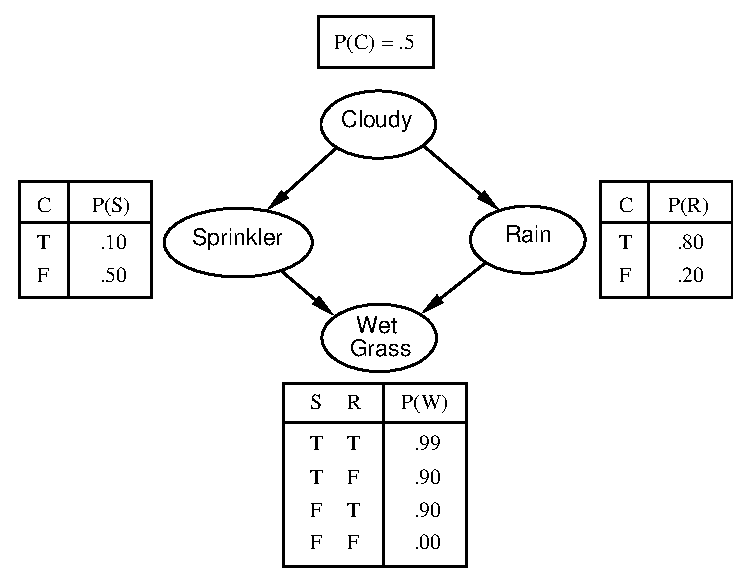
\includegraphics[width=2.2in]{rain_net}
		\end{column}
		\begin{column}{2in}
			\small
			Initial Sample: $\langle \lnot c, s, \lnot r, w \rangle$ \\
			\smallskip
			\pause
			Updating $C$: \\
			\smallskip
			$
			\begin{array}{l@{}l}
			\pause
			\lefteqn{P(c|\EM{mb}(C))} \\
			\pause
			& = \alpha P(c)P(s|c)P(\lnot r|c) \\
			\pause
			& = \alpha \cdot 0.5 \cdot 0.1 \cdot 0.2 = 0.01\alpha \\
			\pause
			\lefteqn{P(\lnot c|\EM{mb}(C))} \\
			\pause
			& = \alpha P(\lnot c)P(s|\lnot c)P(\lnot r|\lnot c) \\
			\pause
			& = \alpha \cdot 0.5 \cdot 0.5 \cdot 0.8 = 0.2\alpha \\
			\pause
			\lefteqn{\mathbf{P}(C|\EM{mb}(C)) = \left\langle 0.048, 0.952 \right\rangle}
			\end{array}
			$ \\
			\smallskip
			\pause
			Random 0.03\pause: $\langle c, s, \lnot r, w \rangle$ \\
			\medskip
			\pause
			\begin{tabular}{@{}llll@{}}
				\bfseries Update & $R$  & $W$  & $C$ \\
				\bfseries Random & 0.48 & 0.63 & 0.83 \\
				\pause
				\bfseries Result & \lefteqn{\langle \lnot c, s, r, w \rangle}
			\end{tabular}
		\end{column}
	\end{columns}
\end{frame}
\begin{frame}{Gibbs Sampling}
	\begin{block}{Properties}
		Given $n$ variables, $s$ samples, and $\leq d$ nodes $\in \EM{mb}(X)$:
		\begin{itemize}
			\item Time Complexity: \pause $O(nds)$
			\pause
			\item Unlike rejection sampling, all samples are used
			\pause
			\item Performs well in practice
		\end{itemize}
	\end{block}
	\pause
	\begin{block}{Problems}
		\begin{itemize}
			\item Difficult to tell when convergence is achieved
			\item Performs worse when Markov blankets are large
		\end{itemize}
	\end{block}
\end{frame}


\part{Key Ideas}
\begin{frame}{Key Ideas}
	\begin{block}{Bayesian Networks}
		\begin{itemize}
			\item Variables linked by conditional independence
			\item Put causes on top, add direct effects below
			\item $P(x_{1},\ldots,x_{n}) = \prod\limits_{i=1}^{n}{P(x_{i}|\EM{parents}(X_{i}))}$
		\end{itemize}
	\end{block}
	\begin{block}{Inference Methods}
		\begin{itemize}
			\item Exact: sum reordering and dynamic programming
			\item Rejection sampling requires many samples
			\item Likelihood weighting poor with a lot of evidence
			\item Gibbs Sampling updates based on Markov blanket
		\end{itemize}
	\end{block}
\end{frame}

\end{document}


